%preámbulo
\documentclass[12pt,oneside,FLEQN]{report}
\usepackage{fancyhdr}
\usepackage[pages=some]{background}
\usepackage{amssymb,amsthm,amsmath,enumerate,graphicx,tabularx}
\usepackage[utf8]{inputenc}
\usepackage[hidelinks]{hyperref}
\usepackage[spanish]{babel}
\usepackage[rflt]{floatflt}
\usepackage{multicol}
\usepackage{tcolorbox, empheq}
\tcbuselibrary{skins,breakable,listings,theorems}
\usepackage{tikz,tkz-tab}
\usetikzlibrary{matrix,arrows, positioning,shadows,shadings,backgrounds,calc, shapes, tikzmark}
\usepackage{subfigure}
\usepackage{caption}
\usepackage[a4paper]{geometry}
\geometry{top=1.5cm, bottom=1.5cm, left=3cm, right=3cm}
\usepackage{ragged2e}
\newcommand{\marcar}[3]{\tikz[overlay,remember picture,baseline=-2pt] \node[circle,#1,draw,text=black, inner sep=1pt] (#2) { #3};}
\parindent=0cm
\usepackage{listings}
\hypersetup{
colorlinks=true,
linkcolor=black,
filecolor=magenta,
urlcolor=cyan,
citecolor=greenwhats
}
\backgroundsetup{
	scale=1,
	color=black,
	opacity=0.4,
	angle=0,
	contents={
\includegraphics[scale=1.5]{Fondoportada.png}}
}
\usepackage[dvipsnames,table]{xcolor}
%\usepackage{lscape}
\usepackage{enumitem}
\definecolor{greenwhats}{RGB}{37, 211, 102}
\definecolor{gris}{rgb}{0.33, 0.41, 0.47}
\usepackage{fancyhdr}
\usepackage{natbib}
\usepackage{colortbl}
\usepackage{array,booktabs}
%\usepackage{pdflscape}
\usepackage{longtable}
\definecolor{codeturquoise}{RGB}{72,202,228}
\definecolor{codeyellow}{RGB}{255,170,51}
\definecolor{codepurple}{RGB}{255, 203, 242}
\definecolor{codegreen}{RGB}{149,213,178}
\definecolor{backcolour}{RGB}{73,80,87}
\definecolor{white}{RGB}{255,255,255}
\lstdefinestyle{estilochidori}{
backgroundcolor=\color{backcolour},
commentstyle=\color{codeyellow},
keywordstyle=\color{codeturquoise},
numberstyle=\tiny\color{codegreen},
stringstyle=\color{codepurple},
basicstyle=\ttfamily\footnotesize\color{white},
breakatwhitespace=false,
breaklines=true,
captionpos=b,
keepspaces=true,
numbers=left,
numbersep=5pt,
showspaces=false,
showstringspaces=false,
showtabs=false,
tabsize=2
}
\lstset{style=estilochidori}
\begin{document}
{
\fontfamily{qag}\selectfont
	\BgThispage
\begin{titlepage}
        \topmargin=1cm
        \centering

        {\bfseries\LARGE Universidad Autónoma de Querétaro \par}
        \vspace{1cm}
        {\scshape\Large  Facultad de Ingenier\'ia  \par}
        \vspace{3cm}
        %\centering
        \begin{figure}[!h]
        	\centering
                
\includegraphics[height=5cm]{Logouaq.png}
        \end{figure}
        \vspace{2cm}
        {\itshape\large Tarea 12: Integración numérica pt.2\par}
        \vspace{3cm}
        {\Huge Análisis numérico\par}
        \vspace{2cm}
        {\Large Autor: \par}
        {\large J.A. Salinas Sánchez \par}
        {\large Abril 2022 \par}
\end{titlepage}
	\clearpage
	\newpage
\tableofcontents
\chapter{Introducción}
Siguiendo con la parte de integración numérica, la indudabilidad del impacto e importancia en el desarrollo de la humanidad del cálculo infinitesimal ha impulsado a matemáticos, físicos y demás personas a buscar manera de resolver integrales numéricas de manera mucho más eficiente, así como más precisa. Es aquí donde entran otros métodos de integración: los métodos compuestos.\\

Los métodos compuestos toman su nombre del simple hecho de que utilizan varios métodos matemáticos (no sólo de integración), como extrapolaciones o interpolaciones, para refinar sus aproximaciones. Entre dichos métodos se tiene los siguientes:
\section{Integración de Romberg}
Este método de integración consiste en combinar el método del trapecio con la extrapolación de Richardson. El primer método ya lo conocemos. El segundo consiste en  obtener $n$ aproximaciones de la integral de la función $f(x)$, $I$,y relacionándolas en pares, obtener $n-1$ aproximaciones; así hasta obtener una última. La manera en la que la integración de Romberg logra aumentar su exactitud, no sólo es por obtener más aproximaciones, sino, poder asignar un peso a cada una; pues, las $n$ aproximaciones de inicio se hace una más exacta que la anterior; mediante el incremento en las iteraciones de dichas aproximaciones. Entonces, tiene en cuenta que el peso de cada aproximanción debe ser mayor que la anterior.  Entonces, el método se divide en dos etapas:
	\begin{itemize}
		\item Obtener las aproximaciones: se obtiene $n$ aproximaciones de I mediante la regla del trapecio compuesta, duplicando el número de iteraciones para cada aproximación subsecuente. 
	\end{itemize} Aplicar la extrapolación de Richardson: es empareja cada aproximación con su subsecuente y se obtiene una nueva aproximación mediante la siguiente fórmula:
	\begin{equation}
		I_{j,k}\equiv \dfrac{4^{k-1}I_{j+1,k}-I_{j,k-1}}{4^{k-1}-1}
	\end{equation}
	Cuando se llegue a una única aproximación, el proceso habrá finalizado.
\section{Cuadratura de Gauss-Legendre}
En el siguiente método, como siempre, Carl Friedrich Gauss tuvo algo que ver. Contemporáneo de éste, el matemático francés Adrien-Marie Legendre había descubierto un grupo de polinomios que satisfacen una cierta ecuación diferencial:
\begin{equation}
	\dfrac{d}{dx}\left[(1-x^{2})\dfrac{d}{dx}P_{n}(x)\right]+n(n+1)P_{n}(x)=0
\end{equation}
Y se pueden calcular mediante la siguiente ecuación:
\begin{equation}
	P_{n}(x)=\dfrac{1}{2^{n}n!}\dfrac{d^{n}}{dx^{n}}\left[(x^{2}-1)^{n}\right]
\end{equation}
Estos polinomios tienen la característica de ser ortogonales entre sí, por lo que se podrían definir como linealmente independientes, así como sus soluciones. Es por eso que se utilzan apliamente en la expansión analítica de funciones, en especial para interpolaciones mediante polinomios, utilizando el concepto de que las todo vector (refiriéndonos a espacios vectoriales) resulta una suma (combinación lineal) e vectores linealmente independientes.\\

Gauss sabiendo esto, los utilizó, no para interpolar; sino para extrapolar datos de una función $f(x)$ a una fórmula de integración fija. Es decir: si, con una interpolación, uno genera una función o más datos a partir de unos ya obtenidos; con una extrapolación (cuadratura), uno ajusta los datos a una función predeterminada (los cuadra). Y eso es lo que hizo Gauss.\\

Gauss se basó en la regla del trapecio; pero, en lugar de escoger dos puntos exteriores del intervalo y de cada subintervalo de integración, planteó utilizar dos puntos interiores. Para ello, panteó cambiar el intervalo de integración de $[a,b]$ a $[1,1]$ mediante la siguiente sustitución:
\begin{equation}
	I=\int_{a}^{b}f(x)dx=\dfrac{b-a}{2}\int_{-1}^{1}f(\dfrac{b-a}{2}u+\dfrac{b+a}{2})du
\end{equation}
Lo que, aplicando suma de Riemann implicaría que:
\begin{equation}
	I\approx\dfrac{b-a}{2}\sum_{i=1}^{n}w_{i}f(\dfrac{b-a}{2}u_{i}+\dfrac{a+b}{2})
\end{equation}
Con $u_{i}$ siendo las raíces del polinomio de Legendre que resulte del número de iteraciones deseadas. Así que Gauss definió que, según el número $n$ que se utilice para aproximar una integral; se puede obtener las raíces del polinomio de Legendre del mismo grado que $n$ como los $x_{i}$ en los que evaluar la función y el peso de cada término de la suma $w_{i}$ mediante la siguiente fórmula:
\begin{equation}
	w_{i}=\dfrac{2}{(1-x^{2})\left[P_{n}(x_{i})\right]^{2}}
\end{equation}
\chapter{Desarrollo y método}
Los problemas se resolvieron de la siguiente manera: se construyó tres códigos: uno para la integración numérica múltiple, otro para la cuadratura de Gauss y otro para la integración de Romberg. Además, se utilizó como apoyo los códigos para interpolaciones mediante polinomios, trabajados anteriormente.\\

El código para la integración de Romberg pide el grado de complejidad al que se quiere llegar $h=2n$; luego, realiza $n$ aproximaciones de $I$ con la regla del trapecio $\dfrac{1}{2}$, duplicando el número de iteraciones hasta llegar a $h$. Finalmente, aplica la fórmula de Romberg hasta reducir todas las aproximaciones a una sola, y devuelve el resultado. \\

Luego; el código de cuadratura gaussiana recibe una función y, dependiendo del $n$ dado, va realizando la sumatoria obteniendo los coeficientes $w_{i}$ y las raíces de los polinomios de Legendre previamente cargados en una lista. Por último, realiza la sumatoria y regresa el resultado.\\

Concluyendo, la integración numérica múltiple se realiza mediante integración trapezoidal simple, primero sobre una variable, y luego, sobre otra.
\section{Código}
	\subsection{Romberg}
	\lstinputlisting{Romberg.py}
	\subsection{Cuadratura Gaussiana}
	\lstinputlisting{Gauss.py}
\section{Problemas}
	\subsection{Unidad 21}
		\subsubsection{21.15}
		\subsubsection{21.23}
	\subsection{Unidad 22}
		\subsubsection{22.1}
		\begin{figure}[!h]
			\centering
			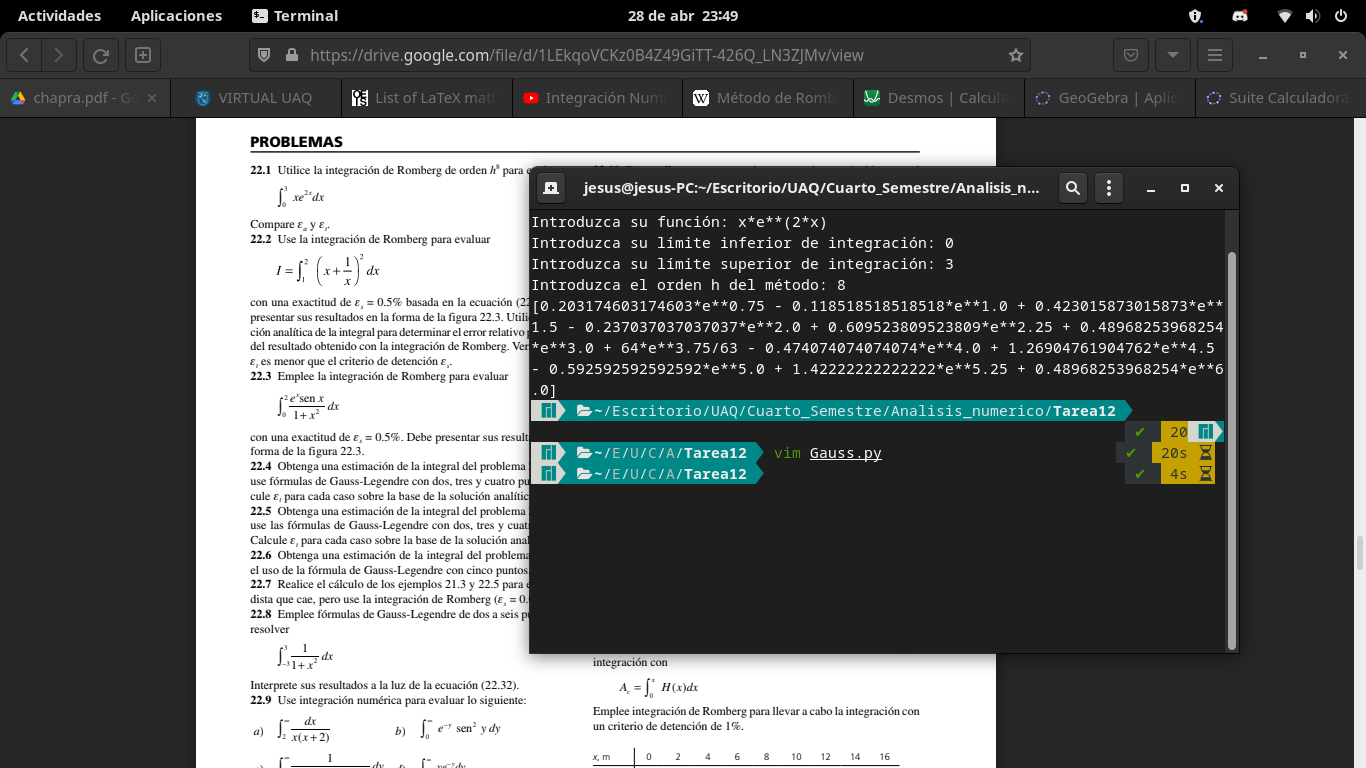
\includegraphics[scale=0.3]{221.png}
			\caption{Resultado del ejercicio 22.1}
		\end{figure}
		\subsubsection{22.5}
		\begin{figure}[!h]
			\centering
			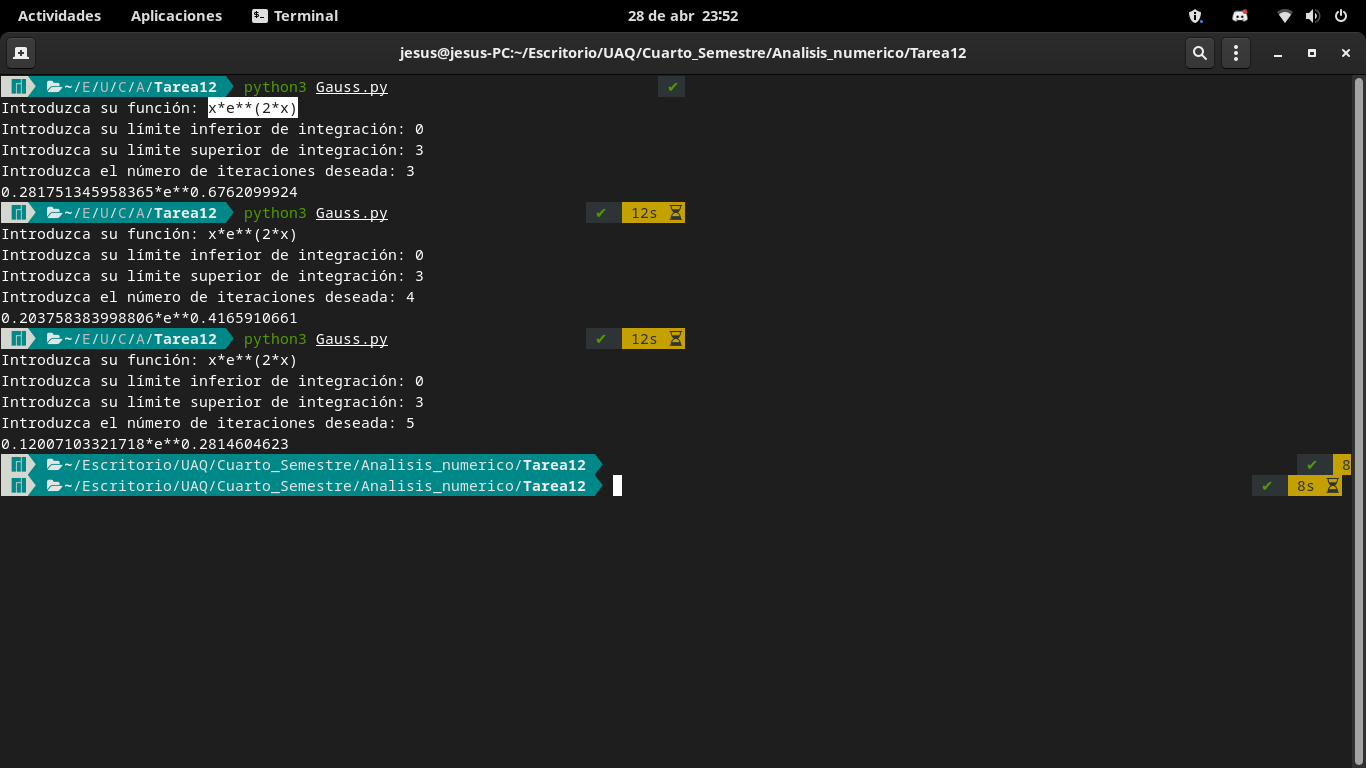
\includegraphics[scale=0.3]{225.png}
			\caption{Resultado del ejercicio 22.5}
		\end{figure}
		\subsubsection{22.9}
\chapter{Conclusión}
Contar con métodos que logren refinar tanto la precisión de las aproximaciones obtenidas mediante otros métodos de integración numérica, con un costo computacional fijo; representa un gran logro del análisis numérico; pues, con los métodos simples de integración numérica, para mejorar los resultados se tiene que incrementar el número de iteraciones hasta que, en algunos casos, ya no es informáticamente costeable hacerlo. En cambio, si uno tiene un métodos con costos computacionales fijos, que se pueden controlar al detalle (como la Cuadratura de Gauss, donde uno hasta puede dejar fijo el número de iteraciones), y con resultados tan buenos; en muchos casos las soluciones numéricas son casi equivalentes a las analíticas. Esto último hace que casi literalmente resolvamos lo irresolvible. 
\begin{thebibliography}{1}
	\bibitem [1]{Chapra} Chapra, S.C. et Canale, R.P (2015) {\it Métodos numéricos para ingenieros} McGrawHill. pp (494-510)

		%494-510
\end{thebibliography}
}
\end{document}
